\documentclass[border=7pt]{standalone}
\usepackage{amsmath,amssymb,bm,mathtools}
\usepackage[fontset=none]{ctex}
\setCJKmainfont{Songti SC}\setCJKsansfont{PingFang SC}
\usepackage{tikz}\usetikzlibrary{arrows.meta,calc,patterns,angles,quotes,decorations.markings,decorations.pathmorphing}
\newcommand{\dd}{\mathop{}\!\mathrm d}
\definecolor{blue}{HTML}{235789}\definecolor{red}{HTML}{BC4B41}
\tikzset{axis/.style={->,>=Stealth,line width=.55pt},world/.style={line width=.9pt},flow/.style={->,>=Stealth,line width=.85pt},ray/.style={->,>=Stealth,line width=.85pt},guide/.style={dashed,line width=.4pt},aux/.style={dashed,line width=.4pt},dim/.style={<->,>=Stealth,line width=.5pt},every node/.style={font=\normalsize},force/.style={->,>=Stealth,very thick},gas/.style={fill=blue!7}}
\begin{document}
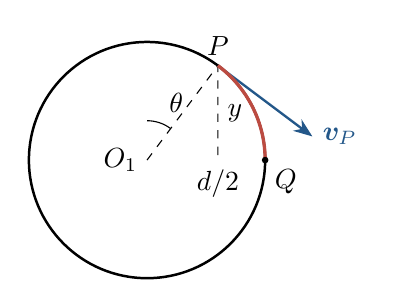
\begin{tikzpicture}\draw[world](0,0)circle(1.5);\draw[guide](0,0)--(.9,1.2)--(.9,0);\node[below]at(.9,0){$d/2$};\node[left]at(0,0){$O_1$};\node[above]at(.9,1.2){$P$};\draw[flow,blue](.9,1.2)--(2.1,.3)node[right]{$\bm v_P$};\node[right]at(.9,.6){$y$};\draw(0,.5)arc(90:53.1301:.5)node[midway,above right]{$\theta$};\draw[red,very thick](.9,1.2)arc(53.1301:0:1.5);\fill(1.5,0)circle(1.2pt)node[below right]{$Q$};\end{tikzpicture}
\end{document}
